\chapter{Determination of the material budget}

  The discovery of new physics and the characterisation of the already known particles are possible only with performant detectors.
  As it was presented on chapter~\ref{chap:vxd}, the fabrication of a vertex detector is constrained by two parameters: the pointing resolution and the material budget.
  The first fully functional prototype of \gls{PLUME} was tested in November 2011 at CERN with 120 GeV pions.
  The results have shown that the pointing resolution of the ladder corresponds to the expected value for the \gls{ILD} and moreover, the use of a double-sided structure improves this pointing resolution. 
  Nevertheless, the material budget ($\rm{X}_0$) of such device is estimated only by calculation and the SPS beam is not suited to a material budget measurement.
  Therefore, a test beam campaign of the PLUME-V1 prototype was done in April 2016 at DESY test beam 21 with positrons up to 5 GeV.
  Firstly, the test beam preparation is discussed.
  Then, the motivation, the test beam facility, as well as the tools used for the analysis are presented.
  Finally, the results on the radiation length measurements are discussed.
  %The reason to test an already known prototype is that the performances have to be the same at low and high-momentum particles.
  %The preparation of the test beam is firstly discussed.
  %Then, the test beam facility, as well as the tools used for the analysis are presented.
  %Finally, the radiation length measurements are discussed..

  %The first fully functional prototype of \gls{PLUME} was tested in November 2011 at CERN with 120 GeV pions. 
  %Due to the environment, the ladder has to be able to track high momentum particles, as well as ones with low momentum.
  %The material budget on the sensitive area for incoming particles is estimated to be about 0.65 \% $X_0$.

\minitoc

  \section{Preparation of the test beam}

  In April 2016, a test beam campaign with electrons and positrons up to 5 GeV was performed at the DESY-II test beam facility.
  The first fully functional PLUME ladder (PLUME-V1) was tested again to study the performances of this device with low-momentum particles.
  The different measurements scheduled are presented here, as well as the preparation of the test beam, from the PLUME integration to the data acquisition.

  % A second test beam was performed in April 2016 at DESY with positrons up to 5 GeV. 
  % The goal of this test beam was to study the performances of this device with low-momentum particles.
  % The ladder tested is a second PLUME-V1 prototype.
  % The steps, from the preparation to the analysis are explained here.
  % Different measurements were planned to fully test the ladder.
  % Nevertheless, as this test beam was at the end of my Ph. D., I could not perform all the measurements.
  % The preparation are presented for all the measurements, but the analysis itself is focused only on the radiation length measurement.

    \subsection{Measurements and telescope configuration}

    During the two weeks of test beam, several measurements were performed to test as mush as possible the ladder.
    The measurements scheduled are: 
    \begin{itemize}
      \item Spatial resolution
      \item Mini-vectors
      \item Deformation study:
      \begin{itemize}
        \item Tilt up to $60^{\degree}$ with a $10^{\degree}$ step
        \item Air flow speed between 3 and $5~\rm{m.s}^{-1}$
      \end{itemize}
      \item radiation length along the sensors and on the mechanical flex
    \end{itemize}

    Although all the planed schedule was performed, the test beam was at the end of my Ph. D., therefore, I was no able to perform all of the measurements.
    The section~\ref{sec:X0} presents the study I have performed on the radiation length measurement.

    The pointing resolution of the telescope depends on the spacing between the different planes. 
    The best resolution is achieved by placing the inner planes of the telescope as close as possible to the \gls{DUT} and the outer planes as far as possible from the \gls{DUT}.
    Because of the deformation study, which needs to rotate the ladder, the inner planes can not be close to the \gls{DUT} without modifying the geometry at each steps.
    Hence, to keep a consistent alignment and to reduce the time spending on the off-line alignment, it was decided to fixed the inner planes as close as possible to be able to rotate the ladder without modifying the geometry.
    Moreover the ladder is not centered in its box, so to keep an equal distance between the two sides of the ladder and the two inner planes, the minimal distance between the telescope planes are calculated by taking into account an offset.

    %The telescope has a better pointing resolution when the inner planes are very close to the \gls{DUT} and the outer planes are far away from it.
    %Nevertheless, to perform the deformation measurements and to tilt the \gls{DUT} without moving the telescope planes at every angle and performing the alignment steps one more time, the two inner planes have a distance of ....
    %Moreover, the ladder is not placed in the middle of the box, thus, the distance between one inner telescope plane to the box is different from the distance between the other side and other telescope plane.

    For the first time, the collaboration has decided to use the EUDET telescope and EUDAQ for the acquisition, instead of the Strasbourg telescope and the IPHC acquisition.
    Several configuration are available for the set-up used.
    The first ones consist to use the six planes of the EUDET telescope and to have two separate acquisition, one for \gls{PLUME} and the second one dedicated for the telescope and then, to merge the data together.
    As the EUDET telescope are equipped with the same sensors as \gls{PLUME}, the acquisition can be simplified by having only four telescope planes and connecting directly two sensors of the \gls{DUT}.
    A simulation toolkit developed by Simon Spannagel and based on \gls{GBL} is used to compare the pointing resolution at the \gls{DUT} position for different telescope geometries.
    Here, the six and four telescope planes set-up are compared for different energies and spacing between the sensors.
    This simulation takes into account the material budget of the telescope, the \gls{DUT} and the multiple scattering of electrons in the air.
    One telescope plane as a material budget of ..., whereas \gls{PLUME} is $0.65~\%$ plus two kapton foils used to insulate the ladder from the light.
    For both configuration, the telescope is divided into two arms, two or three planes on each side of the \gls{DUT}.
    The maximal distance between each plane of one frame is $d_{\rm{max}} = 150~\rm{mm}$ for the six sensors configuration, whereas for the second one it is $d_{\rm{max} = 300~\rm{mm}}$.
    
    \begin{table}[!h]
      \centering
      \begin{tabular}{c c c}
        \hline %----------------------------
        \multirow{2}*{Energy (GeV)} &  \multicolumn{2}{ c }{$\sigma_{\rm{res}}~\rm{(\mu m)}$} \tabularnewline
                              &  4 planes & 6 planes \tabularnewline
        \hline %----------------------------
        \hline %----------------------------
        2 & 4.85 & 4.78 \tabularnewline
        3 & 3.79 & 3.83 \tabularnewline
        4 & 3.35 & 3.40 \tabularnewline
        5 & 3.12 & 3.15 \tabularnewline
        6 & 2.98 & 2.99 \tabularnewline
        \hline %----------------------------
      \end{tabular}
      \caption{Estimation of the resolution measured $\sigma_{\rm{res}}$ at the DUT position for a telescope with four planes and six planes.}
      \label{tab:estimationRes}
    \end{table}

    The table~\ref{tab:estimationRes} summarises the measured resolution at the \gls{DUT} position for different energies and the use of four or six telescope planes does not have an impact on the telescope pointing resolution.
    The figure~\ref{fig:estimationRes4.7GeV} displays the pointing resolution as a function of the different spacing between two telescope planes of the same frame, for an energy set to $4.7~\rm{GeV}$.
    %Several solutions were available.
    %The first one consists to use the six telescope planes of EUDET and a separate acquisition for \gls{PLUME}.
    %As the acquisition is limited to six inputs and the ladder requires at least one sensor on each side to be acquired, a solution to merge the data has to be thought.
    %As the EUDET telescope and \gls{PLUME} are equipped with the same sensors, the acquisition can be simplified by having only four telescope planes and connecting directly two sensors of \gls{DUT}.
    %A simulation tool was used to define which configuration is giving the best pointing resolution at the \gls{DUT} positions.
    %This toolkit was developed by Simon Spannagel and is based on \gls{GBL}.
    %For different energy, the resolution at the PLUME position was calculated for a set-up with four telescope planes and a set-up with six.
    %The material budget of the \gls{DUT} is determined by the material budget of \gls{PLUME} plus two kapton foils used to insulate the ladder from light.
    %For both configuration, the telescope is made of two arms on each side of the \gls{DUT}.
    %With six sensors, the maximal distance between each plane of one frame is $d_{\rm{max}} = 150~\rm{mm}$, whereas for the four sensors configuration it is $d_{\rm{max} = 300~\rm{mm}}$.

   % The results shown on figure~\ref{fig:estimationRes4.7GeV} depicts the measured resolution at the position of the \gls{DUT} as a function of the distance between two telescope planes of the same arm.

    \begin{figure}[!h]
      \centering
      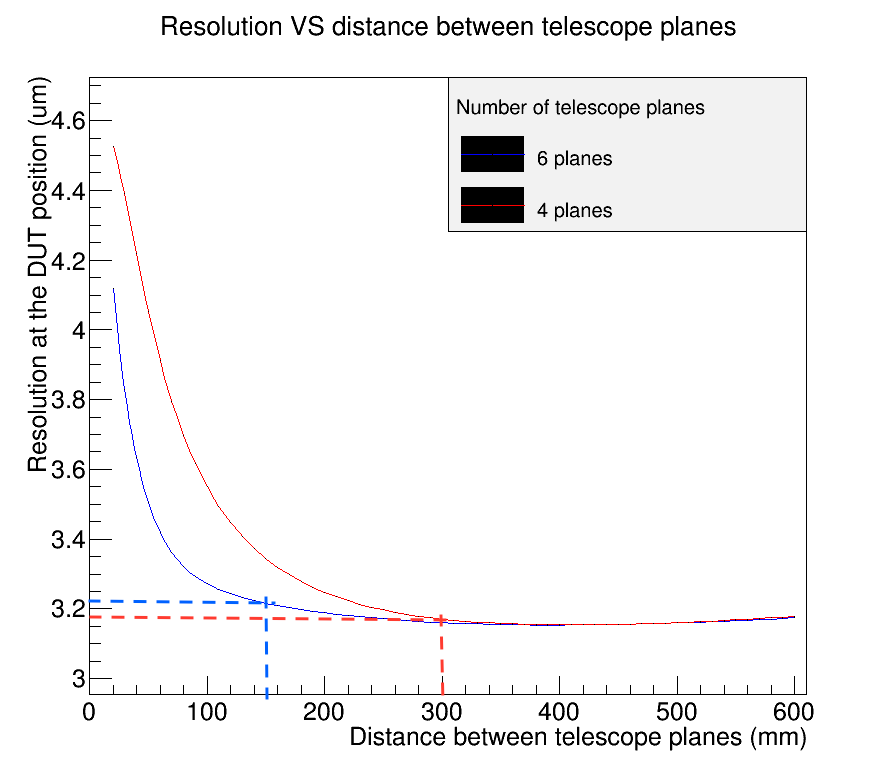
\includegraphics[width = 0.7\textwidth]{Pictures/X0/resolution_4Vs6planes_4-7GeV.png}
      \caption{Estimation of the resolution measured at the DUT position as a function of the distance between two telescope planes of the same arm.
      The blue lines is the results for six planes, whereas the red line is for four planes. 
      The dashed lines are the maximal distance between two planes due to the rail limitation of the telescope frame.}
      \label{fig:estimationRes4.7GeV}
    \end{figure}

    As the number of telescope planes does not impact the pointing resolution, it has been decided to use only four telescope planes to simplify the acquisition system.
    The sensors of the telescope and \gls{PLUME} are both \gls{MIMOSA}-26 thinned down to $50~\rm{\mu m}$.
    Instead of building a DAQ compatible with EUDAQ, two EUDET telescope planes are removed from the set-up and replaced by two \gls{PLUME} sensors (one on each side).
    However, the synchronisation and the stability of the acquisition have to be tested before the test beam campaign. 

    \subsection{Acquisition system}
      
      \subsubsection{EUDAQ}

      EUDAQ is a modular cross-platform data taking framework developed for the EUDET-type beam telescopes\cite{Jansen}.
      It is designed to be flexible and to have an easy integration of other devices.
      The software is based on \textit{producers}, that are link between the different subdetector systems, such as the beam telescope, the \gls{DUT} user DAQ and the \gls{TLU}.
      The events are built by the \textit{Data Collector}.
      All subdetectors events are correlated to form one single global event for data belonging to one trigger.
      
      To simplify the acquisition system, only one DAQ is used, but the robustness of the acquisition has to be tested. 
      Hence, multiple tests are performed in the lab to make sure that EUDAQ is working with \gls{PLUME} and then, single MIMOSA-26 sensors are added to the set-up.

      \subsubsection{Hardware}

      After ensuring that there is no data lose and the acquisition is stable for hours, the integration of \gls{PLUME} on the test beam facility as been investigating.
      To perform the deformation studies, the \gls{DUT} has to be on a rotation stage. 
      With respect to the \gls{DUT} coordinate system, the rotation is along the $u$-direction. 
      Two options to perform the rotation are possible.
      The first one consists to have the same orientation between the \gls{PLUME} sensors and the telescope planes.
      Hence, the ladder is in the horizontal position and the rotation needs a complicated frame...
      For the second options, ladder is positioned on the vertical direction. 
      There is a $90^{\circ}$ rotation between the telescope sensors and the \gls{PLUME} ones.
      The frame consists of an aluminum plate insulated on which the \gls{DUT} sits.
      Clamps are used to reduce the force applied by the cable on the flex to avoid to damage the \gls{DUT} during the test beam.
      A plate with screws hold the ladder strongly to the frame.
      The frame is then mounted onto a rotation stage, which is mounted on a translation stage.
      The figure~\ref{fig:mechanics} shows a schematic model of the frame designed and built at DESY.
      
      \begin{figure}
        \centering
        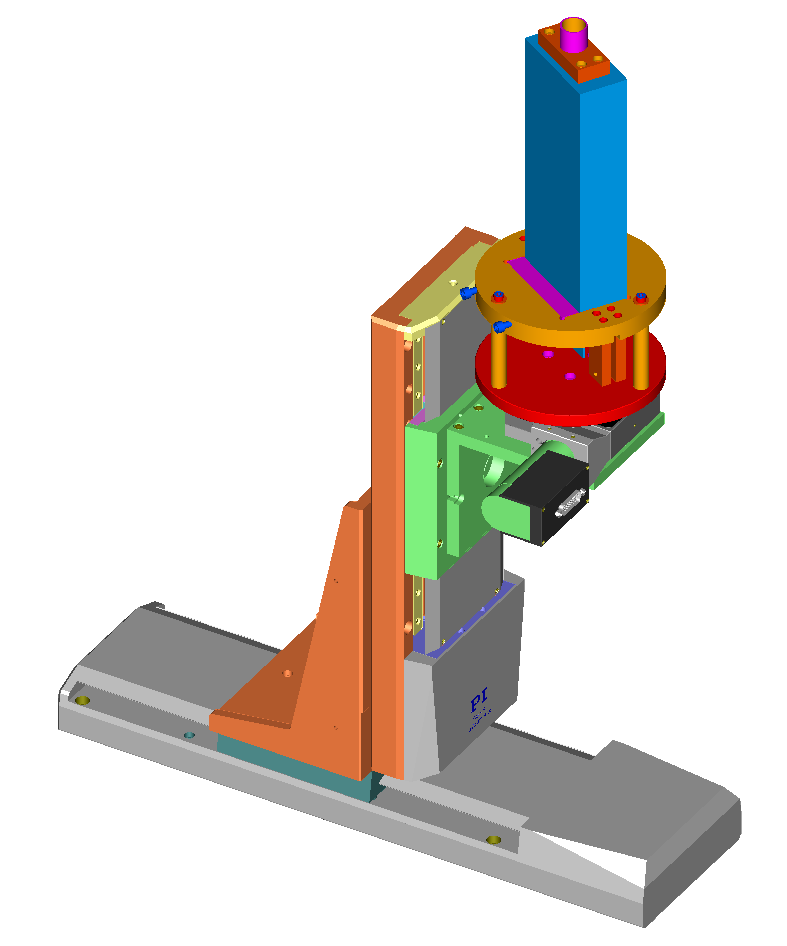
\includegraphics[width = 0.6\textwidth]{Pictures/X0/Frame/Testbeam1.PNG}
        \caption{TCAD model of the mechanical structure designed for the test beam in April. The ladder is hold on a circular frame fixed to a PI rotation stage, mounted onto a XY-table.}
        \label{fig:mechanics}
      \end{figure}

      A cooling system is adapted to maintain a constant temperature. 
      On one endcap, a pipe is fixed and connected to a fan.
      Some studies in Strasbourg were done to determine the air flow speed as a function of the voltage applied.
      Hence, an air flow speed of $3~\rm{m.s^{^1}}$ is achieved with $5~\rm{V}$ and an air flow speed of $6~\rm{m.s^{-1}}$ for $10~\rm{V}$.

      During the test beam campaign, the \textit{clock} and \textit{marker} are read from one sensor of the \gls{PLUME} module.
      The \textit{clock} is extended with a $80~\rm{cm}$ long cable to ensure that one frame starts on the rising edge.
      The second input of the acquisition is a second \gls{PLUME} sensor, followed by the four telescope planes. 
      \gls{PMT}s are placed in coincidence on each side of the telescope to avoid to trigger on fake events where the electrons does not pass through the entire set-up.

      %To ensure the synchronisation of the ladder and the telescope planes, the acquisition is synchronised on the \textit{clock} provided by one of the \gls{PLUME} sensor.
      %In the lab, two MIMOSA-26 sensors and the ladder to test are plugged together to the NI-crate. 
      %Runs of several hours are launched to verify the synchronisation.
      %As the \gls{DUT} and telescope planes are connected to the same \textit{JTAG} card and \textit{clock} distribution board, the start signal arrives at the same time on each sensor.
      %If a delay appears, there is a loss in the synchronisation and the acquisition does not work anymore.
      %The frame-counter should be the same on each sensor.

    \begin{figure}
      \centering
      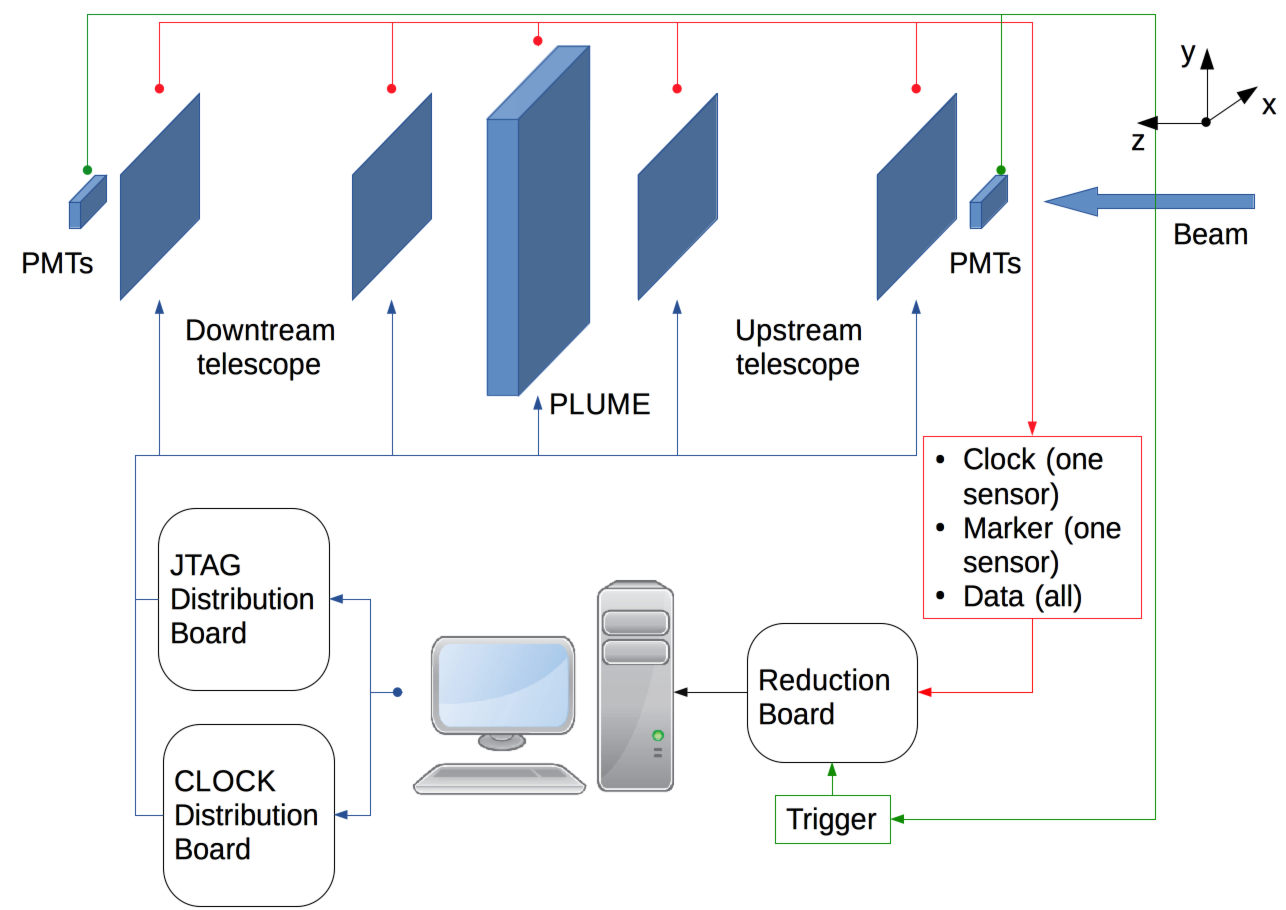
\includegraphics[width = \textwidth]{Pictures/X0/testBeamAcquisition.png}
      \caption{Schematic of the test beam set-up. The PMTs are used for triggering. The clock and marker are read from only one sensor, here it comes from one PLUME sensor.}
      \label{fig:testBeamAcq}
    \end{figure}

    \subsection{experimental set-up}

    %To integrate the ladder onto the translation stage available at the test beam area, a frame was designed and built by the DESY workshop.
    %The ladder is placed vertically a round plate mounted onto a rotation stage. 
    %The figure~\ref{fig:mechanics} shows a schematic layout of the mechanical structure designed and built for the test beam.

    To cool the ladder, a air cooling system is used. 
    It consists of a fan connected to the back endcap of the PLUME box, via a pipe. 
    A measurement performed by Strasbourg gives the corresponding air flow speed to the selected voltage input.  

    \begin{figure}
      \centering
      \includegraphics[width = 0.8\textwidth]{Pictures/X0/testBeam.png}
      \caption{Test beam set-up.......}
      \label{fig:testBeam}
    \end{figure}

    \subsection{Software analysis chain}

    The analysis framework used is called EUTelescope\todo{REF TO EUTEL}.
    It is based on the MARLIN framework from the ILCSOFT.
    It handles LCIO data format.
    Each step of the analysis is driven by dedicated processors.

    The first step consists to convert the raw data files into LCIO data format.
    This file contains the pixel number which fired in a given event, along with the sensor number.
    Then, the noisy pixel are removed before to use a cluster algorithm to form sets of cluster from the individual activated pixels.
    From the cluster information, the hit position is determined by a centre-of-gravity 

    The specific acquisition which is done with EUDAQ has complicated the analysis.
    EUTelescope is coded to expect six telescope planes and a or several \gls{DUT} but at different $z$-positions.
    One way to overcome this problem is to perform a biased analysis. 
    Instead of performing the alignment of the telescope and followed by the \gls{DUT} alignment, the procedure can be done in one way.
    Nevertheless, for an unknown reason GBL and Millepede-II are not working.

    A prototype software based on GBL and Millepede-II and written by Claus Kleinwort has permitted to perform the alignment, as well as the other measurements.
    The software reeds a lcio file containing the hit position of every plane.

    Due to the specific acquisition which was done with EUDAQ, the analysis was a bit complicated.
    EUTelescope was coded to expect six telescope planes plus a single DUT.
    One way to overcome this problem was to perform a biased analysis.
    Instead of performing the alignment of the telescopes and then the DUT for an analysis, this step has to be done in one way.
    Nevertheless, the alignment procedure was not working.

    To perform the alignment, I have used a python script written by Claus Kleinwort, which reads the hit position of every sensor and use GBL and MP-II to perform the alignment.

    %\begin{figure}
    %  \centering
    %  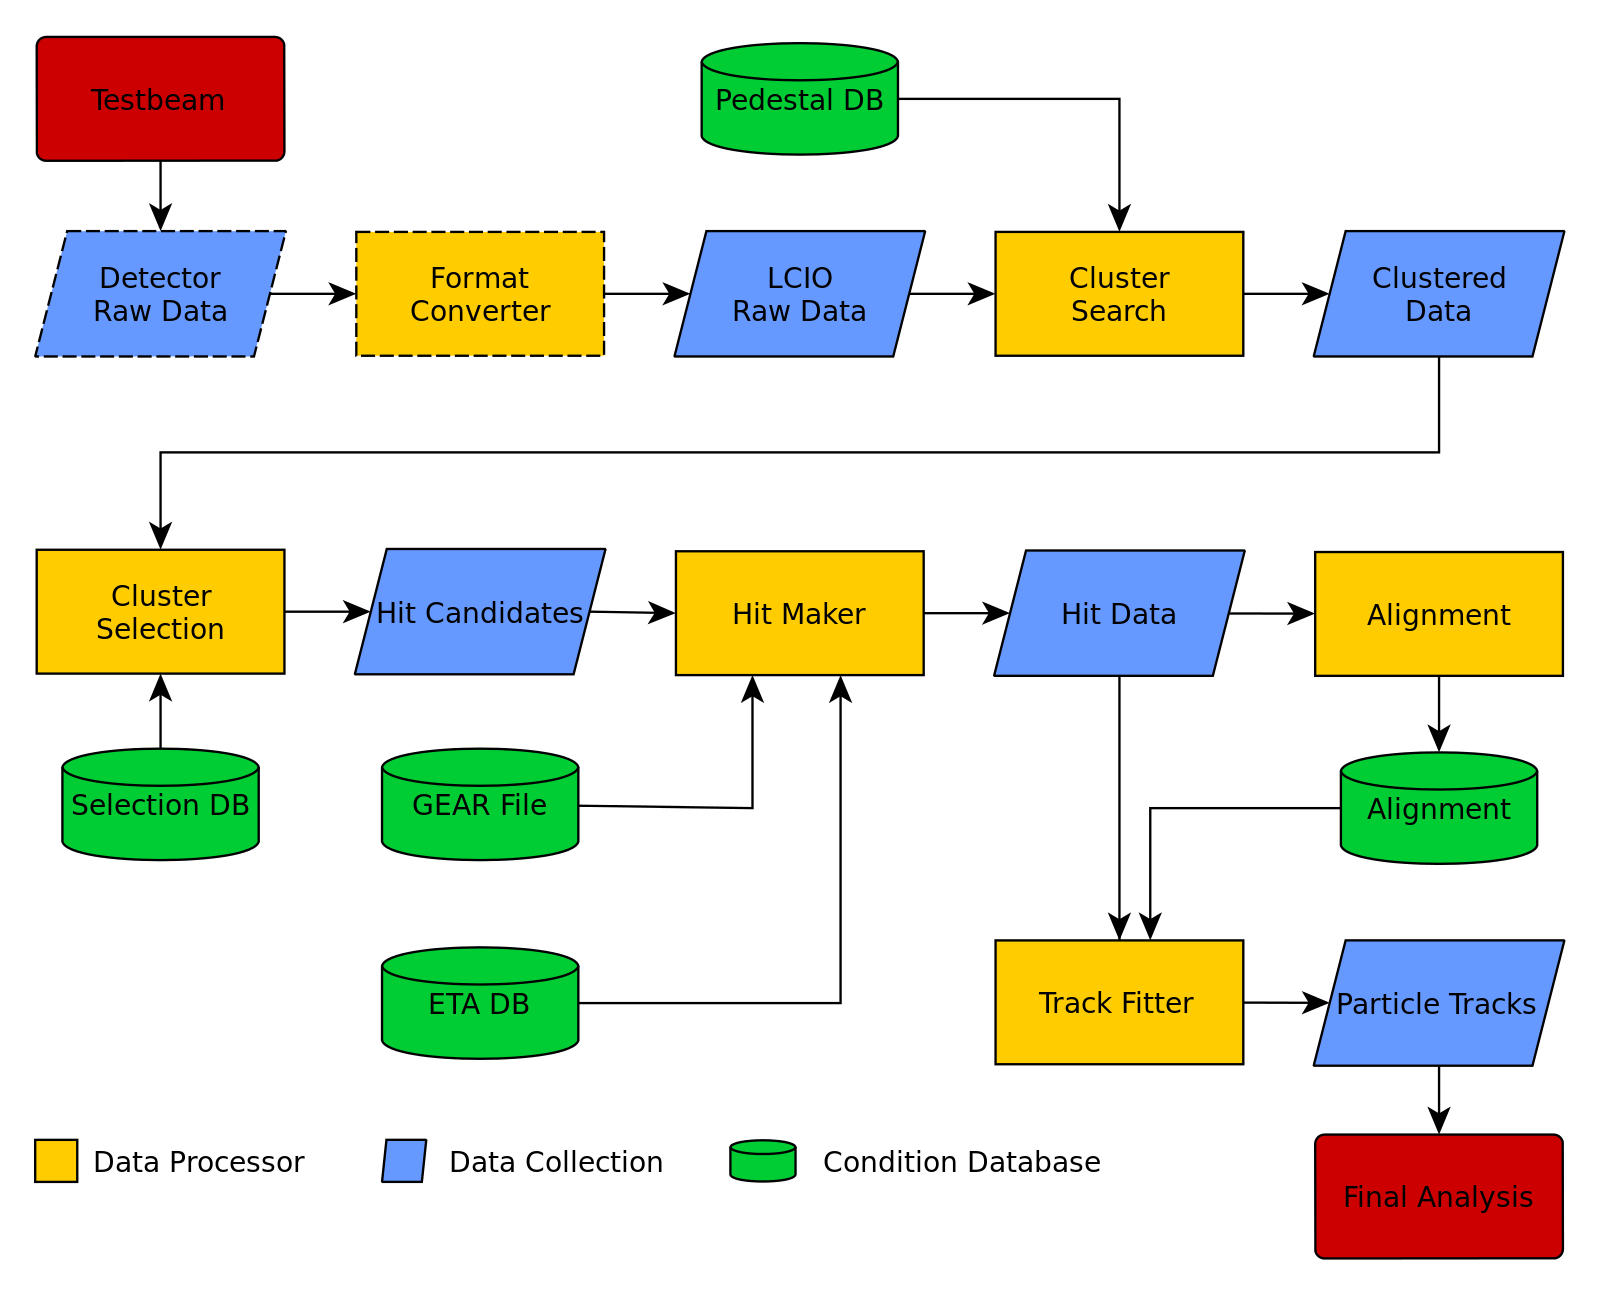
\includegraphics[width = \textwidth]{Pictures/X0/eutel-strategy.png}
    %  \caption{blabla}
    %  \label{fig:eutel-strategy}
    %\end{figure}

  \section{Measuring the radiation length}

    \subsection{Introduction}

    Charged particles travelling through matter lose energy via inelastic collision with atomic electrons, but they also suffered from repeated elastic coulomb scattering from nuclei.
    Thus, they are deflected by many small angles from their initial trajectory because of the multiple coulomb scattering.

    Highland formula describes the projected angle of the incoming particle depending on its momentum $p$, its velocity $\beta c$, its charge number $z$ and its true path length in radiation length unit $\frac{x}{X_{0}}$.

    \begin{equation}
      \theta_{0} = \frac{13.6~\rm{MeV}}{\beta c p} z \sqrt{\frac{x}{X_{0}}}\left(1 + 0.038 \ln{\frac{x}{X_{0}}}\right)
    \end{equation}

    A modified version of the equation describes the electron scattering better than the Highland formula, with $\beta c = 1$ \cite{GEANT4}:

    \begin{equation}
      \theta_{0} = \frac{13.6~\rm{MeV}}{p}\left(\frac{x}{X_{0}}\right)^{0.555},
    \end{equation}

    The spread angle $\theta_{0}$ depends on the momentum $p$ of this particle and the relative radiation length $\frac{x}{X_{0}}$.
    Hence, higher is the momentum, lower is the spread angle. 
    As well, the relative radiation length has an impact on the kink angle. 

    \subsection{Motivation}

    The material budget of a detector is an important aspect during its design.
    The \gls{ILC} sets new goals for the material budget of the vertex detector, but also for other parts of the detector.
    As a reminder, the tracking system should detect precisely the particles path without degrading their energy, while the calorimeters have to measure accurately the energy deposited by the particles.
    To reconstruct accurately the events during a physics analysis, the energy loss inside the different component of the detectors before the calorimeters has to be known, in order to correct the measured energy.

    The radiation length $\rm{X_{0}}$ is the amount of matter traversed by the electron and its unit is $\rm{g}~{cm}^{2}$.
    It is defined as the mean distance over which a charged particle loss $1/e$ of its energy by bremsstrahlung.

    \begin{equation}
      \frac{1}{X_{0}} = \sum_{j} \frac{\omega_{j}}{X_{j}}
    \end{equation}

    \subsection{The DESY II test beam facility}

    The test beam facility at the \gls{DESY} is made of three areas.
    Firstly, the electron beam is produced in the LINAC-II and accelerated to 450 MeV before to be injected in the DESY-II synchrotron ring.
    The DESY-II is used as a storage ring for the PETRA-III. 
    The beam is accelerated and the particles are stored until enough particles are available to be sent on to PETRA, where they are used for photon science.
    
    \begin{figure}[!h]
      \centering
      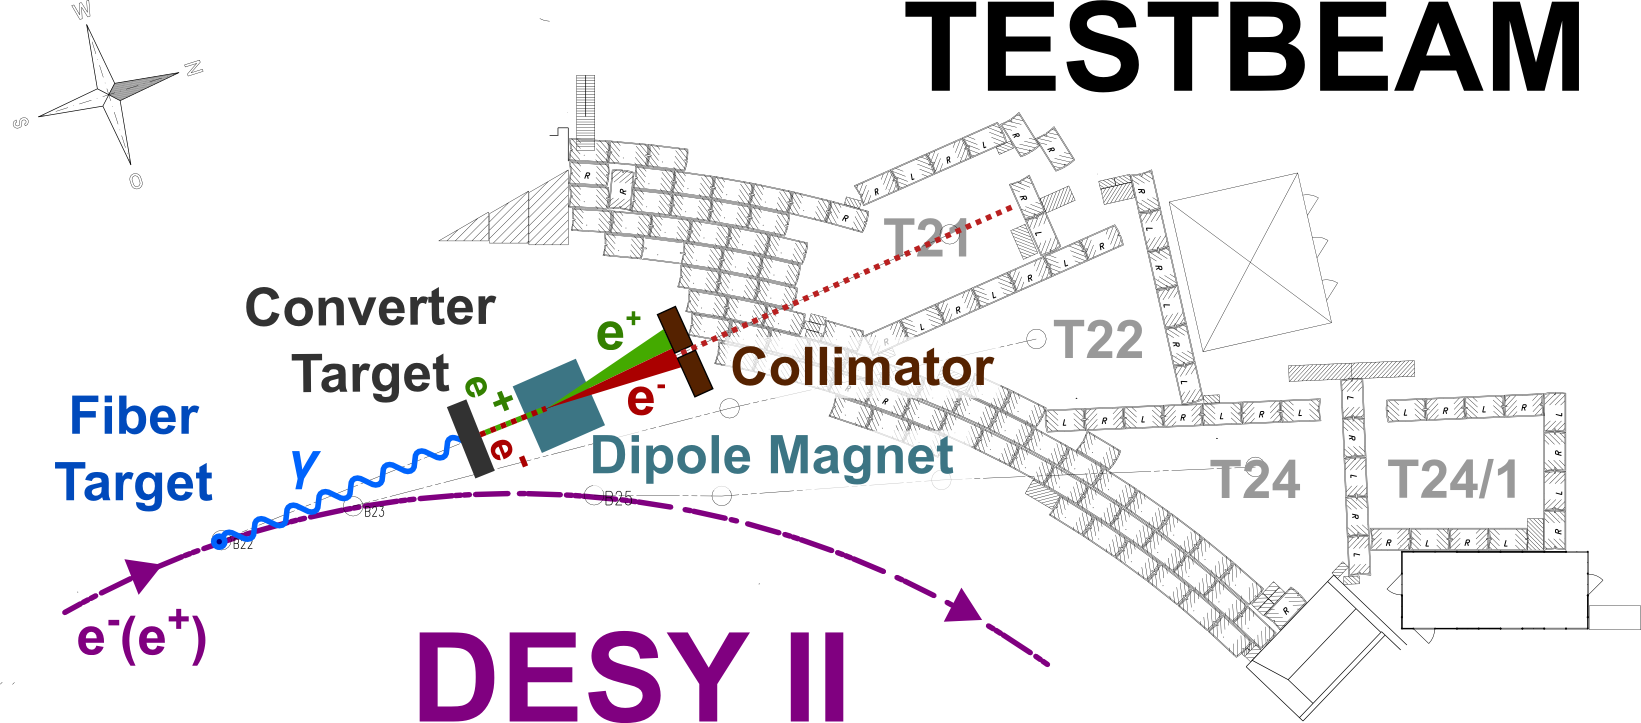
\includegraphics[width = 0.8\textwidth]{Pictures/X0/desy_tb-sketch.png}
      \caption{Schematic layout of the DESY-II test beam facility\cite{DESYII}.}
      \label{fig:desyTb-sketch}
    \end{figure}

    To generate the beam delivered in the Hall 26, a graphite fiber target is placed inside the beam pipe.
    While the electrons are hitting the target, they lose energy and emit bremsstrahlung photons.
    The photons travel through the air and hit a target, on which the photons are converted to pairs of electrons and positrons.
    Different targets with different thicknesses are available and this will impact the particles rate.
    One is made of copper, whereas the other one is made of aluminum.
    Then, a dipole magnet bends the particles and spread them according to their energy.
    Afterward, a tungsten collimator cuts away the unwanted particles, those having a too high or too low momentum, before the test beam area.
    A second collimator is located in the test beam area and it determines the size of the beam spot.
    The figure~\ref{fig:desyTb-sketch} summarises the different step to generate a beam of electrons or positrons in test beam 21, while the energies and the rates available are displayed in figure~\ref{fig:rateTB21}

    \begin{figure}[!h]
      \centering
      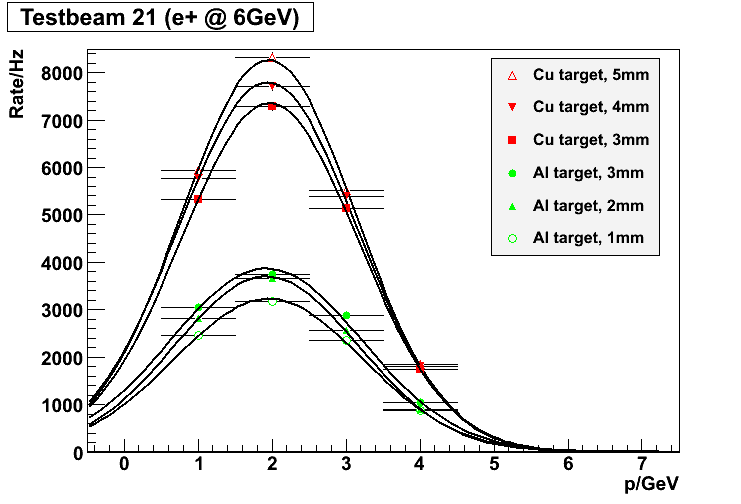
\includegraphics[width = 0.8\textwidth]{Pictures/X0/rate_vs_p_t21.png}
      \caption{Rate for different momentum and with different converter targets\cite{DESYII}.}
      \label{fig:rateTB21}
    \end{figure}


  \section{Analysis}
